\indent\textbf{Fantasia3D}~--~There are several ways to initiate the generation of 3D models in Fantasia3D. The most straightforward method, used in this section, is to begin with just the prompt, wherein Fantasia3D defaults to using a sphere as the initial mesh, shaping the training process from this starting point. Alternatively, one can customize the sphere's initial values  \([0.5, 0.5, 0.5]\) to better represent the desired object by adjusting the parameters to correspond to \([depth, width, height]\). The final approach involves initializing the mesh with a custom~.obj file, providing a rough outline of the intended shape. An example of the latter approach can be seen in Figure~\ref{fig:generationFantasia2} in the appendix, where the generation process was started with a rough human figure.

\begin{figure}[H]
    \centering
    % Subfigure for textual description
    \begin{subfigure}[b]{0.20\textwidth}
        \centering
        \fontsize{9pt}{7pt}\selectfont\text{Iteration = 0}\vspace{3cm}
        \fontsize{9pt}{7pt}\selectfont\text{Iteration = 5000}\vspace{2.85cm}
        \fontsize{9pt}{7pt}\selectfont\text{Iteration = 10000}\vspace{1.95cm}
    \end{subfigure}
    \begin{subfigure}[b]{0.20\textwidth}
        \centering
        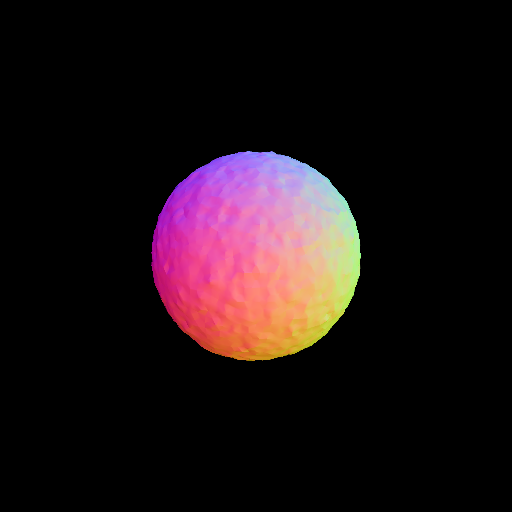
\includegraphics[width=\textwidth]{etc/a robot made out of plants/fantasia3d/fantasia_coarse_robot_0_part2.png}
        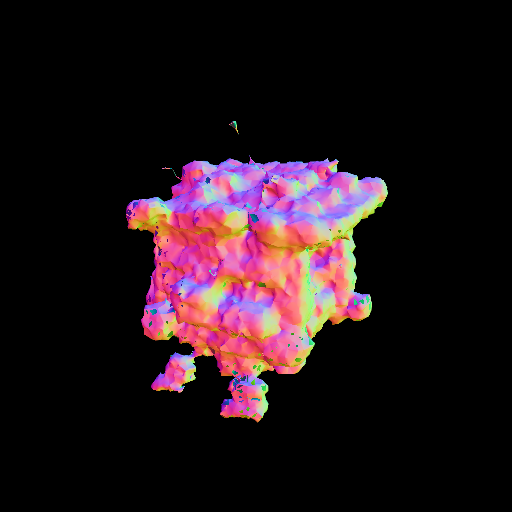
\includegraphics[width=\textwidth]{etc/a robot made out of plants/fantasia3d/fantasia_coarse_robot_5000_part2.png}
        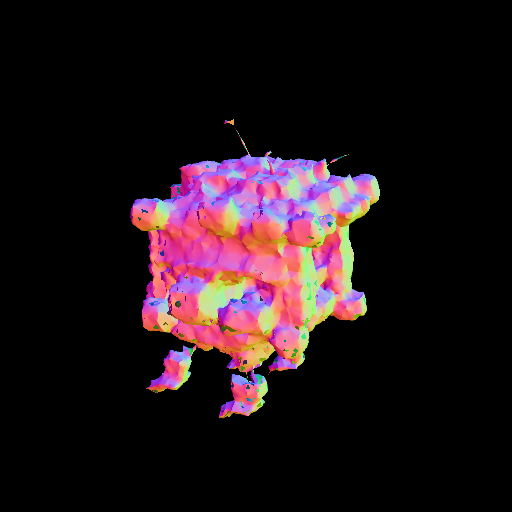
\includegraphics[width=\textwidth]{etc/a robot made out of plants/fantasia3d/fantasia_coarse_robot_10000_part2.png}
        \caption{}
    \end{subfigure}
    \begin{subfigure}[b]{0.20\textwidth}
        \centering
        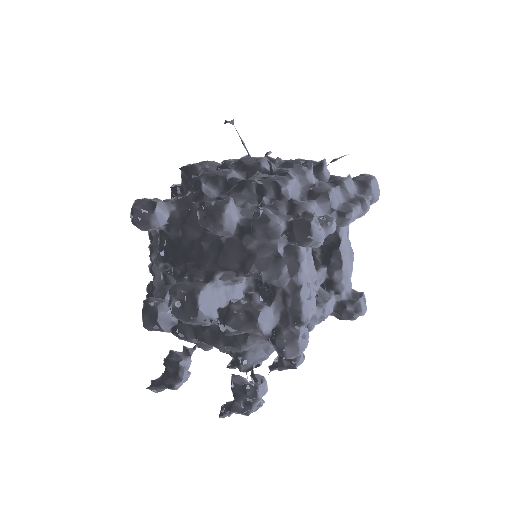
\includegraphics[width=\textwidth]{etc/a robot made out of plants/fantasia3d/fantasia_refine_robot_0_part1.png}
        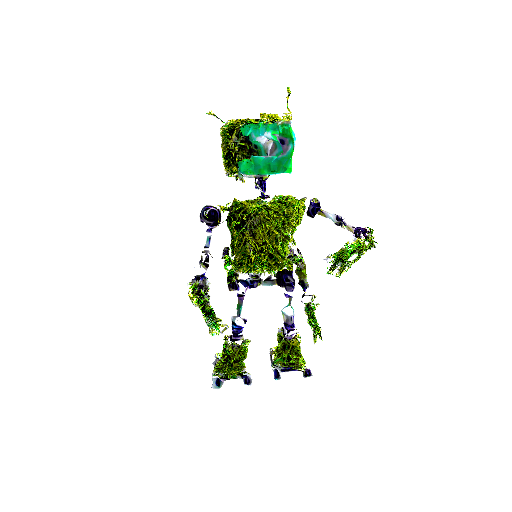
\includegraphics[width=\textwidth]{etc/a robot made out of plants/fantasia3d/fantasia_refine_robot_5000_part1.png}
        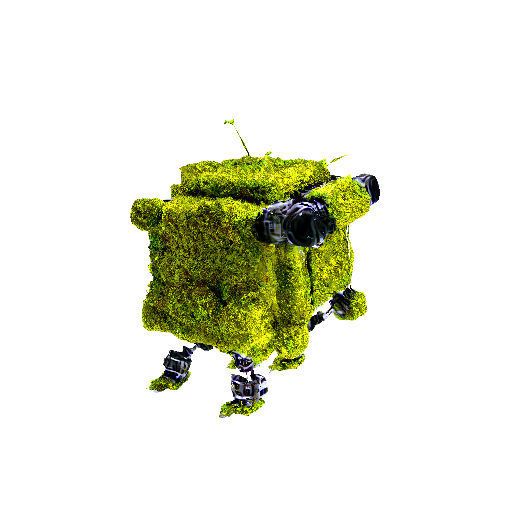
\includegraphics[width=\textwidth]{etc/a robot made out of plants/fantasia3d/fantasia_refine_robot_10000_part1.png}
        \caption{}
    \end{subfigure}
    % Subfigure 3
    \begin{subfigure}[b]{0.37\textwidth}
        \centering
        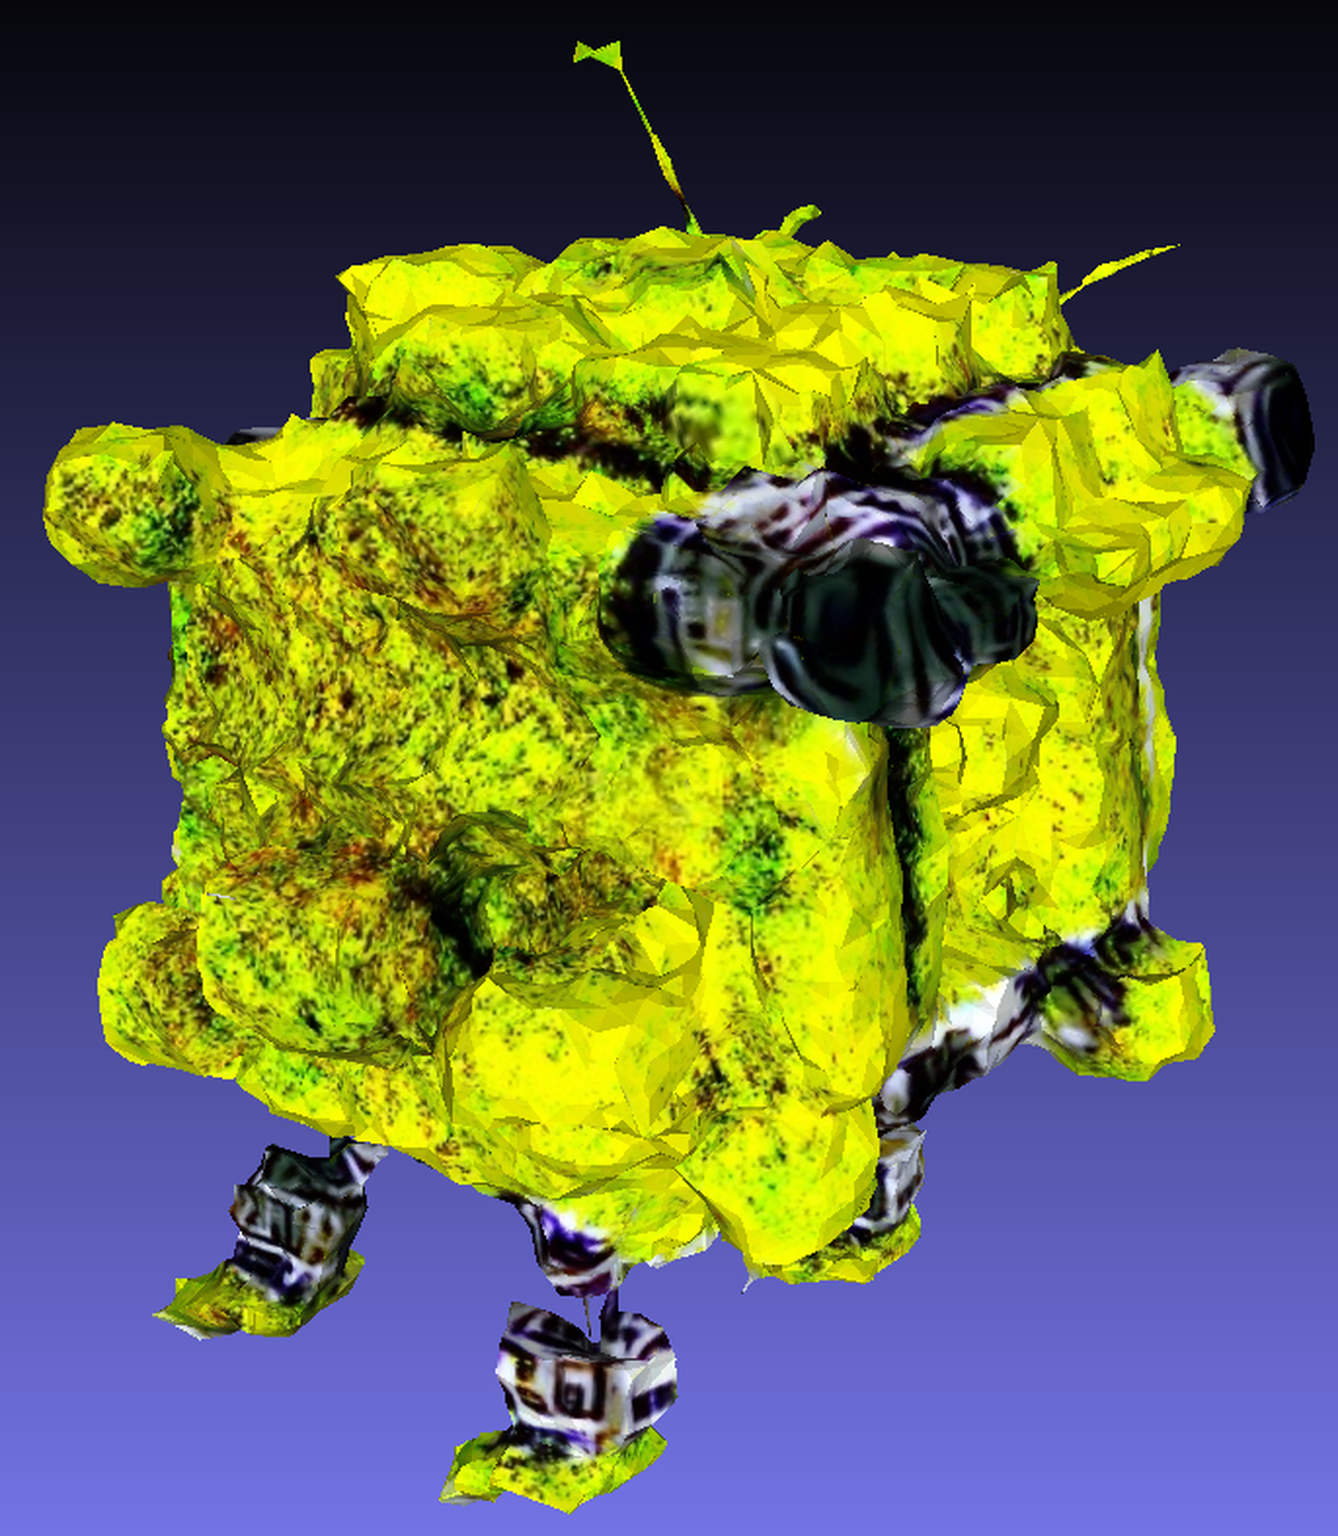
\includegraphics[width=\textwidth]{etc/a robot made out of plants/fantasia3d/fantasia_plantrobot_model_resized.png}
        \caption{}
    \end{subfigure}
    \caption{a: Fantasia3D starting with only a perfect square and refining this according to the prompt ``a robot made out of plants''. In b: only the appearance of the model gets refined. Image c shows the rendered model }~\label{fig:generationFantasia}
\end{figure}

Part (a) of Figure~\ref{fig:generationFantasia} illustrates the geometry stage of the method. Since only the prompt was used for initialization, Fantasia3D automatically selected a sphere as the base, influencing the overall quadratic shape of the final model. The figure reveals that the majority of the transformations occur between iterations 0 and 5000, where the sphere evolves, gaining corners and forming smaller blobs at the bottom, potentially interpreted as the robot's feet. However, at this geometry stage, it's challenging to discern the robot, especially as one made of plants. The changes from iteration 5000 to 10000 are more subtle, with slight smoothing in certain areas, such as the blob on the top left side of the robot or parts of the left foot, but these alterations are not significantly transformative.

Part (b) of the figure displays the appearance stage, where the model is textured. Starting with a greyscale base derived from the previous stage, the model gains color and texture as iterations progress. By iteration 5000, the texture, surprisingly resembling grass, enhances the model's detail and color, diminishing the prominence of the earlier clunky geometry. From iteration 5000 to 10000, this texture is further refined, introducing more detailed color variations and shadows, simulating light effects. Additionally, certain areas of the model exhibit metallic grey tones, particularly noticeable at the top right side and between the main body and the feet. 

However, some of these textural details are lost in the final mesh extraction, as seen in part (c). The model takes on a more yellowish hue, and the previously distinct lighting and shadows are reduced. Similar to the geometry stage, the final model does not clearly represent a robot made of plants; it more closely resembles a box with feet, akin to robots designed for food delivery. Throughout the training, Fantasia3D also generates various textures, including diffuse, roughness, metallic, and normals, as depicted in Figure~\ref{fig:texturesFantasia}.

\begin{figure}[H]
    \centering
      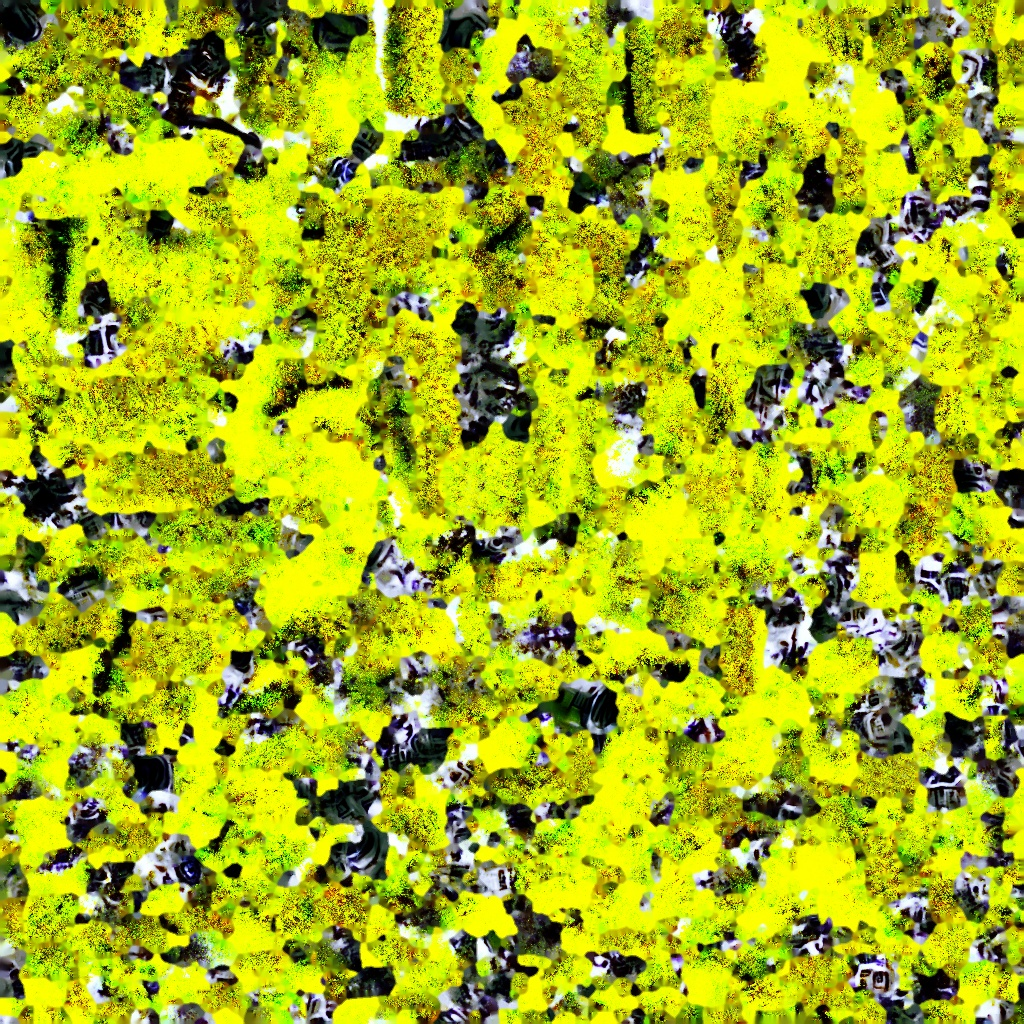
\includegraphics[width=.15\columnwidth]{etc/a robot made out of plants/fantasia3d/fantasia_refine_robot_kd}
      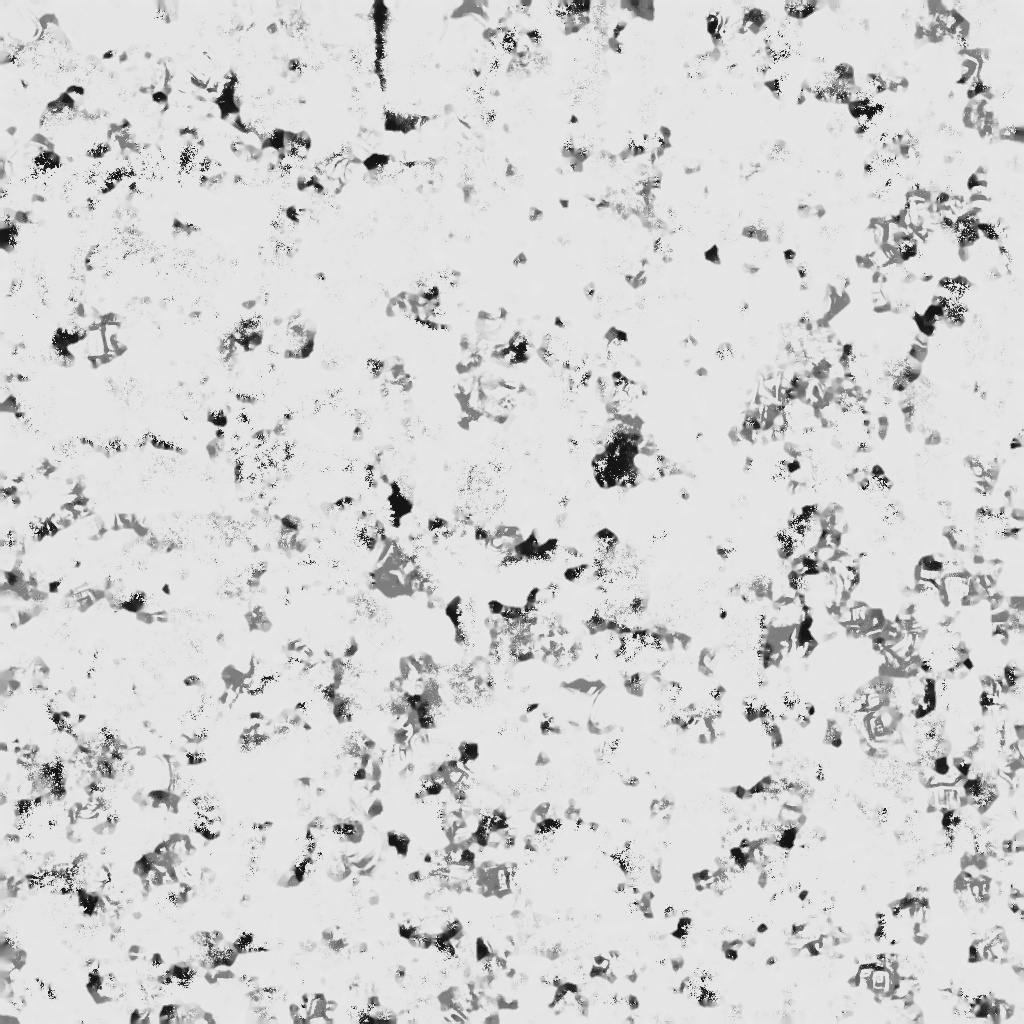
\includegraphics[width=.15\columnwidth]{etc/a robot made out of plants/fantasia3d/fantasia_refine_robot_roughness}
      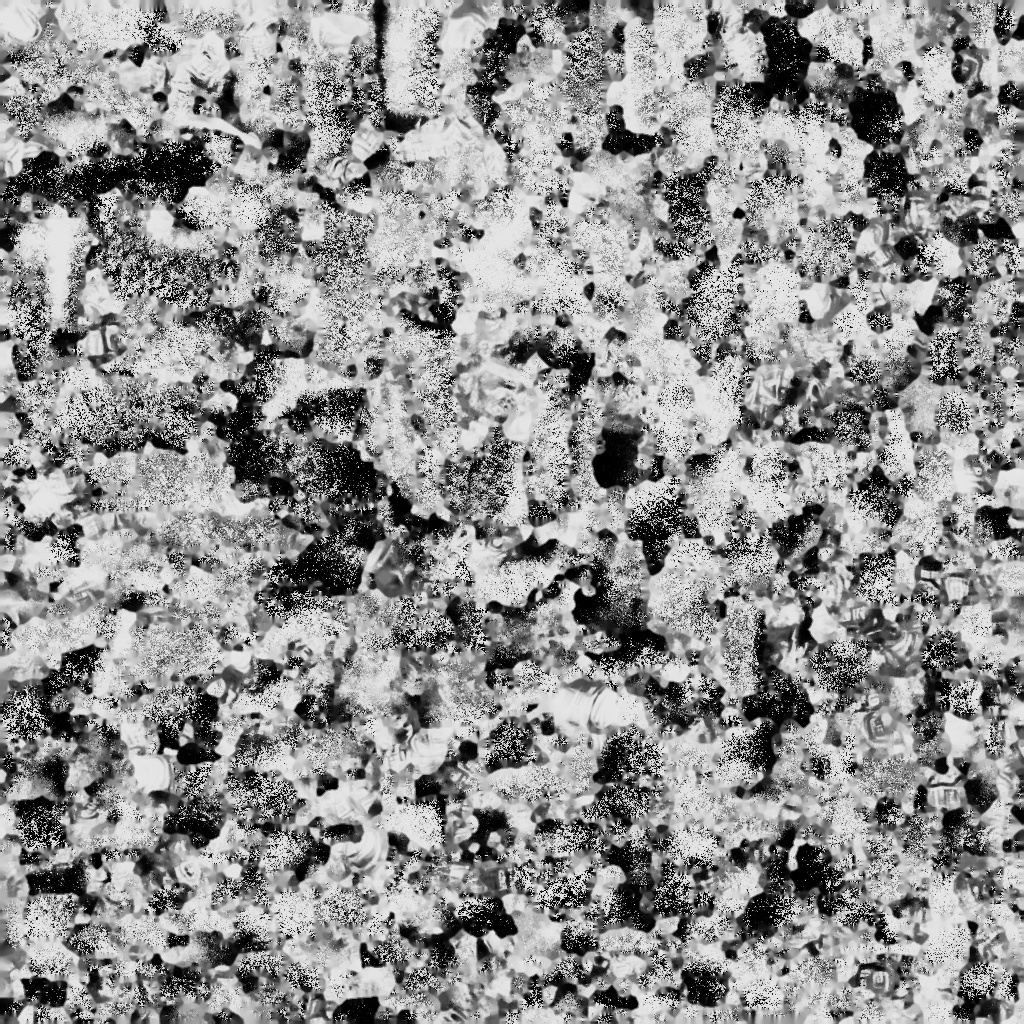
\includegraphics[width=.15\columnwidth]{etc/a robot made out of plants/fantasia3d/fantasia_refine_robot_metallic}
      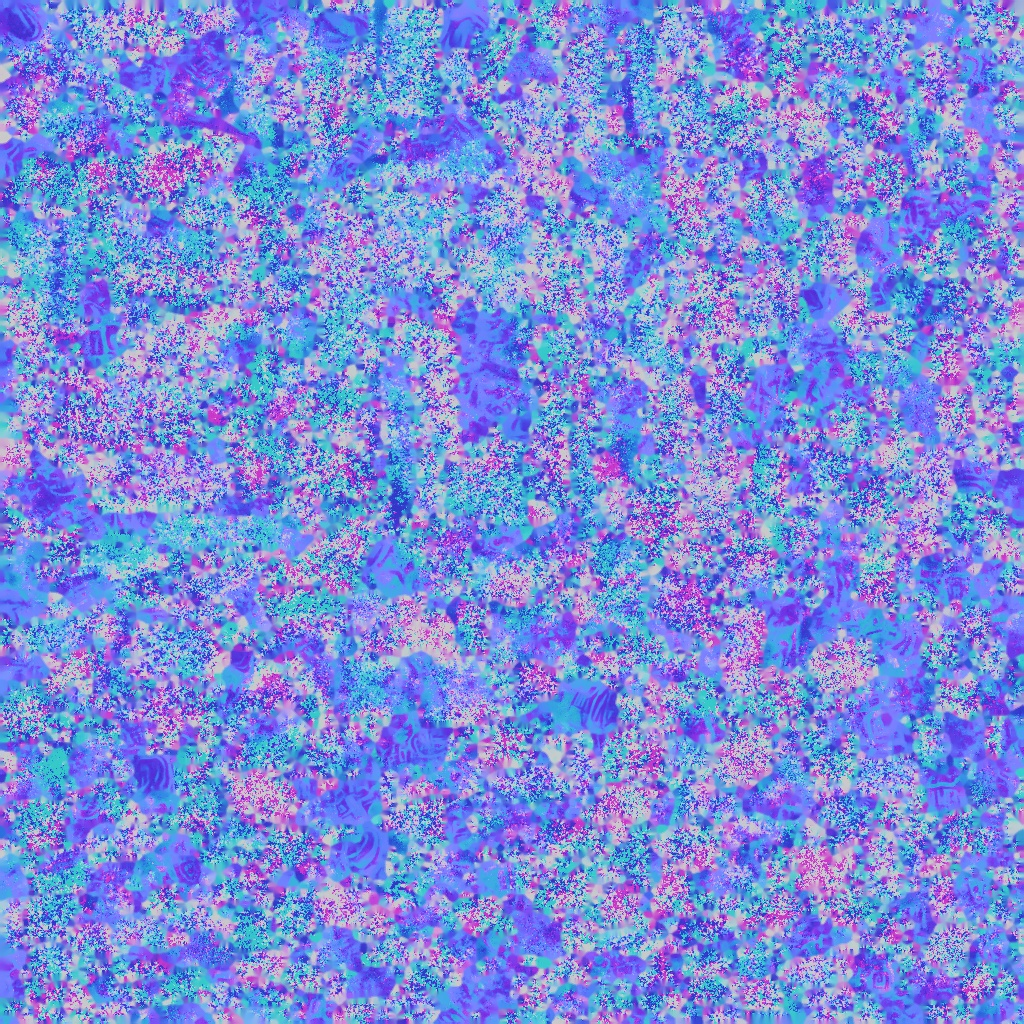
\includegraphics[width=.15\columnwidth]{etc/a robot made out of plants/fantasia3d/fantasia_refine_robot_normal}
      \caption{Generated textures from Fantasia3D\@; from left to right:  diffuse, roughness, metallic, and normal.}~\label{fig:texturesFantasia}
  \end{figure}